\documentclass[norsk,a4paper,12pt]{article}
\usepackage{graphicx}
\usepackage[utf8]{inputenc}
\graphicspath{ {Bilder/} }
\usepackage{hyperref}
\usepackage{commath}
\usepackage{float}
\usepackage{mathtools}


\usepackage[T1]{fontenc}
\begin{document}
\title{Linær regresjoni}
\author{Eirik vetle Winnness}
\maketitle 

\section*{Abstract}

\section*{Introduction}
I dette prosjektett skal jeg se på hvordan de tre forjellig mtodene OLS, ridge, og Lasso best greier å etterligne den ekte fuksjonen(Frankfuksjon). Linær regresjon er en metode man kan bruke for å kunne spå hvordan ny data vil oppføreseg, basert på gammel data. Jeg skal studere MSE(), R2, Bias, og. Jeg har skal studere random data ved å genere det i python programmet ankonda og dens pakker. Jeg skal så se på de fire faktorene og studere OLS, ridge og Laso som om de funger anerldes. Om noen de metodene er bedre til å etterligne datan. jeg kommer til å bruke trenings data for å lage en model, så ser jeg om denne modellen tilppaser seg godt opp mot den virklig fuksjonen. 
\section*{Teori}

\[ MSE(y,\hat{\widetilde{ y}}) =\frac{1}{n}\sum^{n-1}_{i=0}(y_i -\widetilde{ y_i})^2\]
\[ R2(y,\hat{\widetilde{ y}}) =1-\frac{1}{n}\frac{\sum^{n-1}_{i=0}(y_i -\widetilde{ y_i})^2}{\sum^{n-1}_{i=0}(y_i - \bar{y_i})^2} \]
Gjennomsnittet av $\hat{y}$ er definert som:\[\bar{y} =\frac{1}{n}\sum^{n-1}_{i=0}(y_i)\]
\[\bar{y} =\frac{1}{n}\sum^{n-1}_{i=0}(y_i)\]




\subsection*{ Ordinary Least squar}
\subsection*{ Ridge Regression}
\subsection*{Lasso Regression}
\section*{ Ordinary Least squar}

\begin{figure}[H]
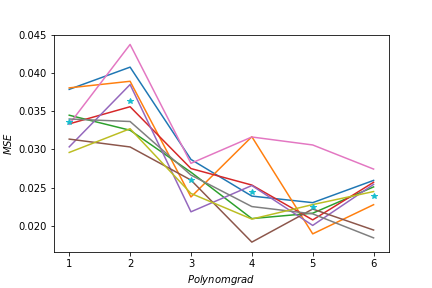
\includegraphics[width=100mm]{MSE}
\caption{Rød(posetivt lad)  blå er negativt lad  }
\end{figure}


\begin{figure}[H]
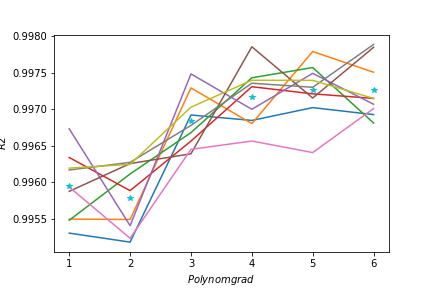
\includegraphics[width=100mm]{R2}
\caption{Rød(posetivt lad)  blå er negativt lad  }
\end{figure}

\begin{figure}[H]
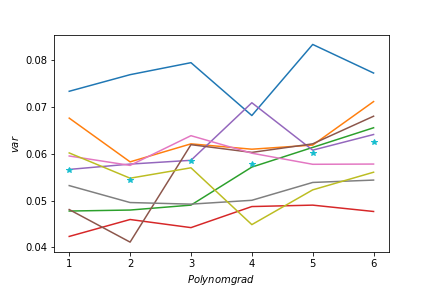
\includegraphics[width=100mm]{var}
\caption{Rød(posetivt lad)  blå er negativt lad  }
\end{figure}

\begin{figure}[H]
\includegraphics[width=100mm]{Bias}
\caption{Rød(posetivt lad)  blå er negativt lad  }
\end{figure}


\section*{ Ridge Regression}
\begin{figure}[H]
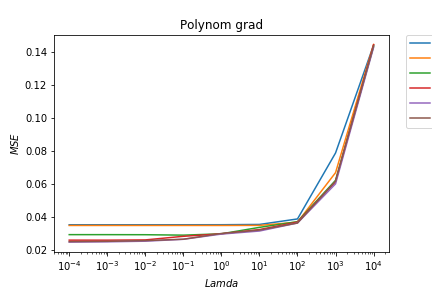
\includegraphics[width=100mm]{MSE(R)}
\caption{Rød(posetivt lad)  blå er negativt lad  }
\end{figure}


\begin{figure}[H]
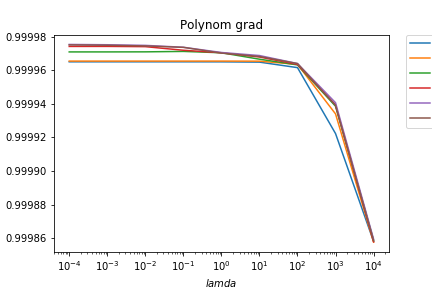
\includegraphics[width=100mm]{r2(R)}
\caption{Rød(posetivt lad)  blå er negativt lad  }
\end{figure}

\begin{figure}[H]
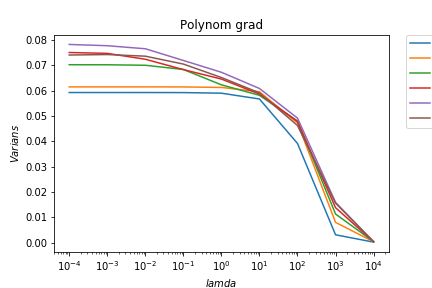
\includegraphics[width=100mm]{var(R)}
\caption{Rød(posetivt lad)  blå er negativt lad  }
\end{figure}

\begin{figure}[H]
\includegraphics[width=100mm]{Bias(R)}
\caption{Rød(posetivt lad)  blå er negativt lad  }
\end{figure}

\section*{Lasso Regression}


\begin{figure}[H]
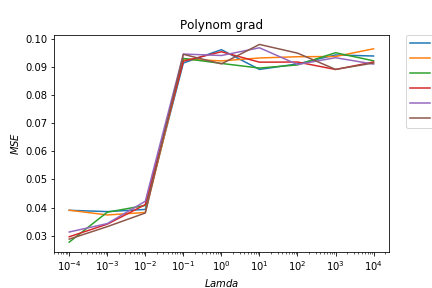
\includegraphics[width=100mm]{MSE(L)}
\caption{Rød(posetivt lad)  blå er negativt lad  }
\end{figure}


\begin{figure}[H]
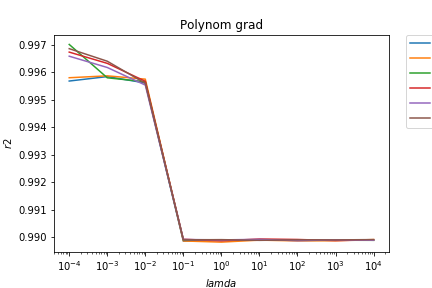
\includegraphics[width=100mm]{r2(L)}
\caption{Rød(posetivt lad)  blå er negativt lad  }
\end{figure}

\begin{figure}[H]
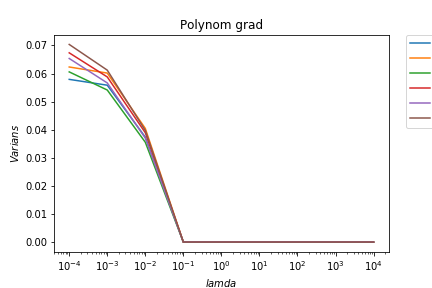
\includegraphics[width=100mm]{var(L)}
\caption{Rød(posetivt lad)  blå er negativt lad  }
\end{figure}

\begin{figure}[H]
\includegraphics[width=100mm]{Bias(L)}
\caption{Rød(posetivt lad)  blå er negativt lad  }
\end{figure}

\section*{Real data}

\section*{konklusjon}
\end{document}